% **************************************************************************** %
\clearpage
\section{Specifications}
\label{appendix:specs}
% **************************************************************************** %

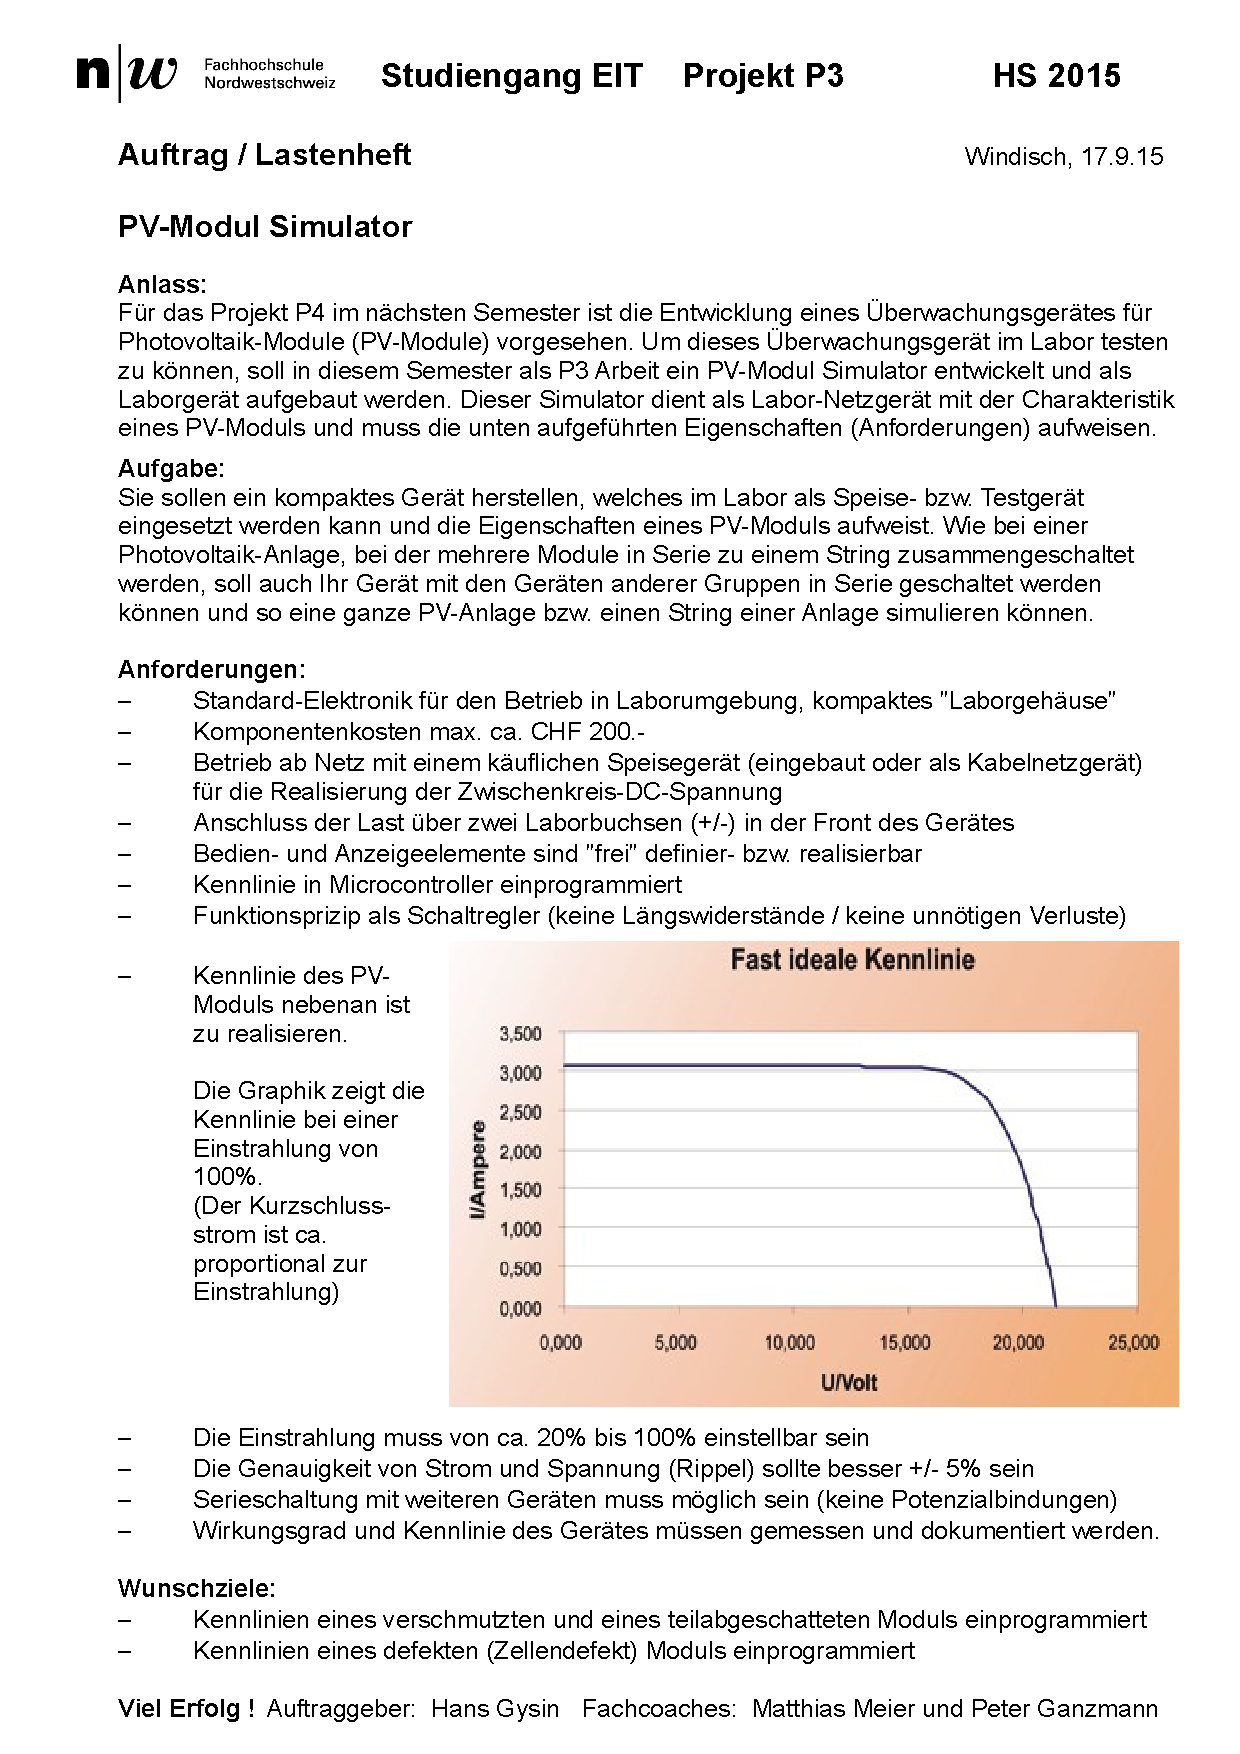
\includepdf[pages=-,scale=1]{images/specs.pdf}
%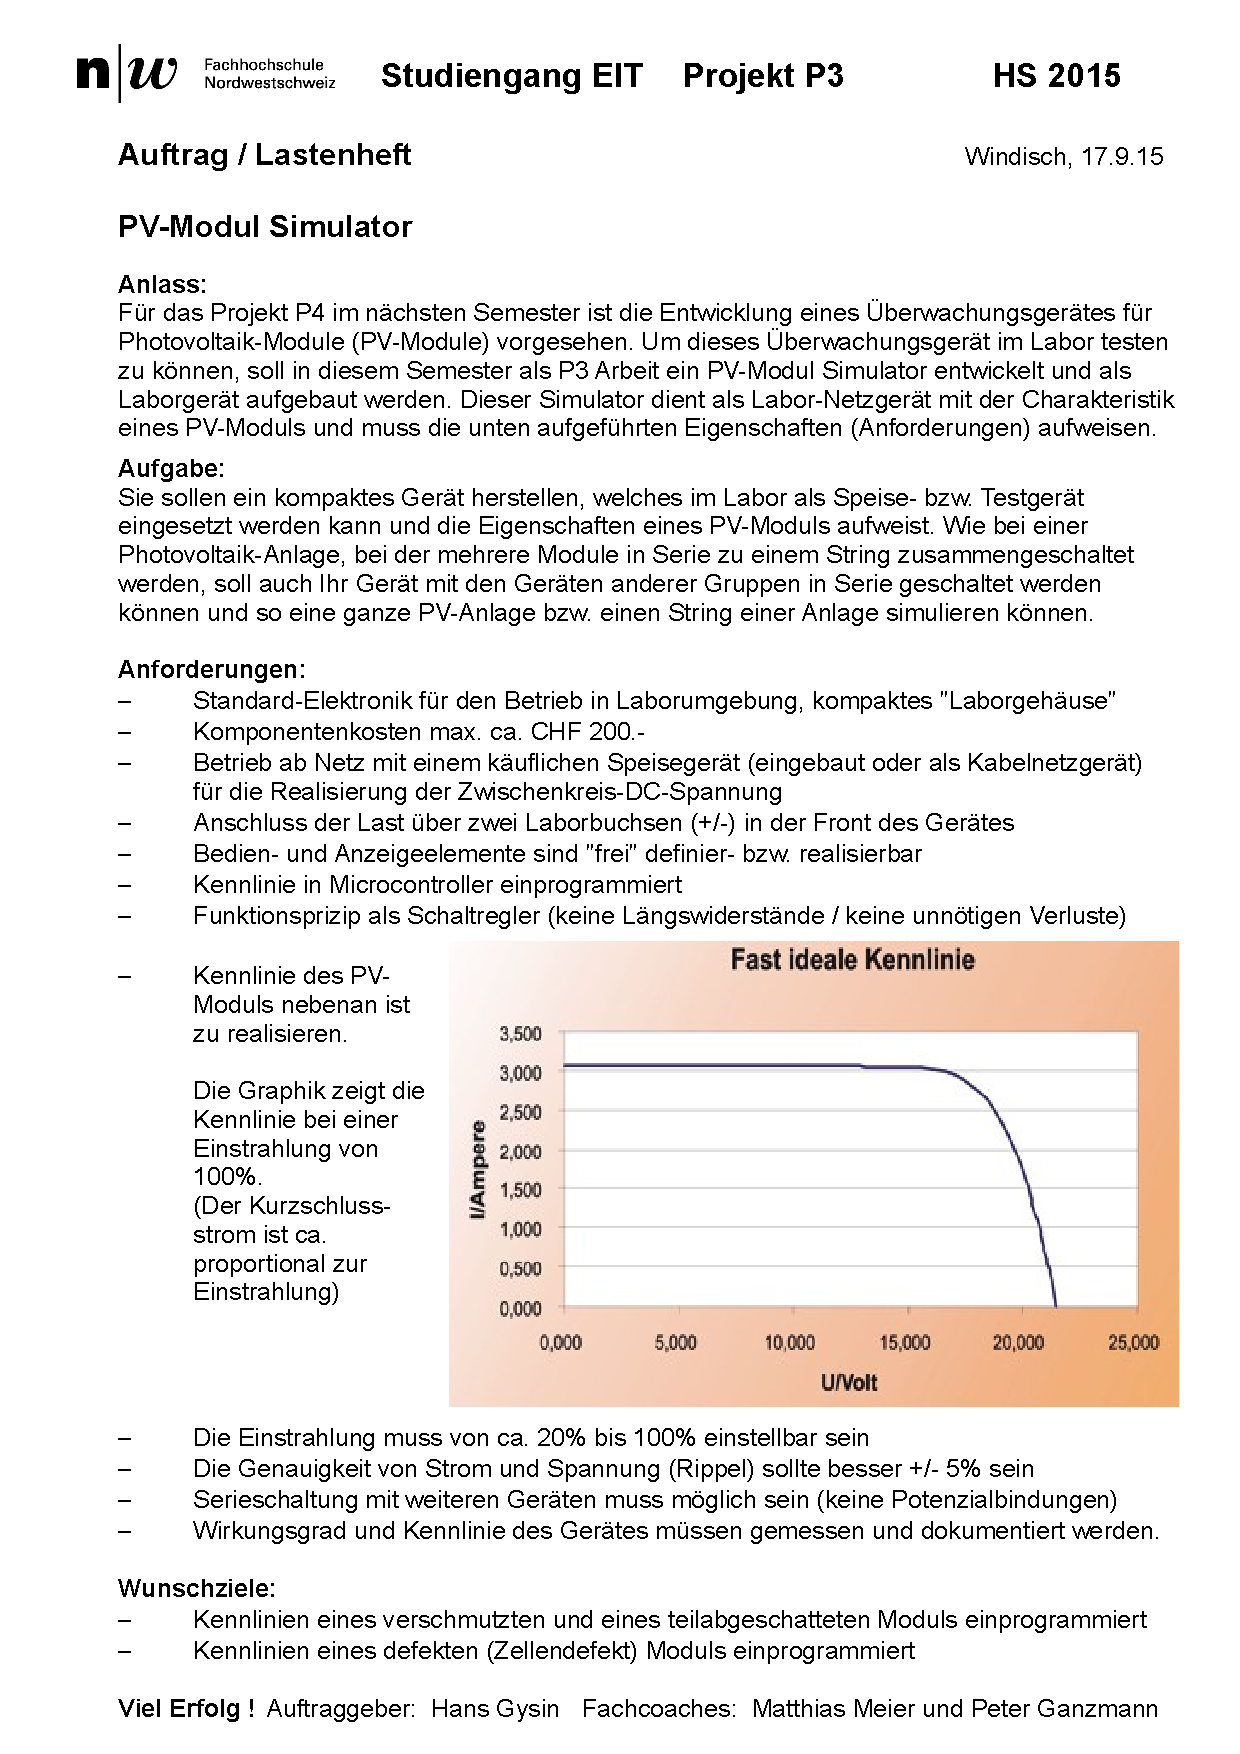
\includegraphics[width=\paperwidth]{images/specs.pdf}

{%START A3 PAGES
    \clearpage
    \pdfpagewidth=2\pdfpagewidth
    \textwidth=2\textwidth
    \addtolength{\textwidth}{50mm}

    % **************************************************************************** %
    \section{LT3471 Circuit}
    \label{appendix:lt3741:circuit}
    % **************************************************************************** %

    \begin{minipage}[b]{.45\textwidth}
        The   circuit    used   to    control   the   LT3471    is   described
        in   detail   in   section  \ref{subsec:lt3741}   starting   on   page
        \pageref{subsec:lt3741}. For the  reader's convenience,  the schematic
        in Figure \ref{fig:circuit:buck} is intended to be folded out and kept
        open as  a reference while  reading that section of  this report. This
        allows  for easy  cross-checking  between text  and schematic  without
        needing to constantly scroll through  the report's pages or needing to
        insert multiple copies of Figure \label{fig:circuit:buck}.
    \end{minipage}%
    \begin{minipage}[b]{.55\textwidth}
        \center
        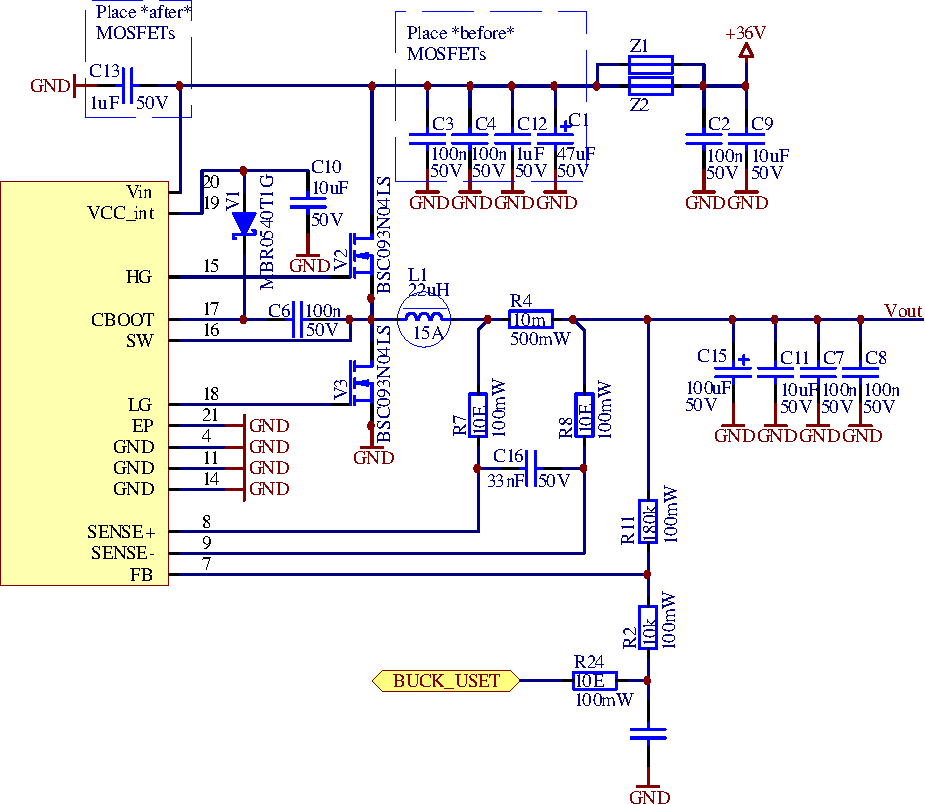
\includegraphics[width=.67\textwidth]{images/circuit/buck.pdf}
        %\caption{Herzst\"uck des Projektes: Aufbau des LT3741 CVCC Synchronwandler}
        \captionof{figure}{The device's heart: Overview of circuit for the LT3741 CCVC synchronous converter.}
        \label{fig:circuit:buck}
    \end{minipage}

\clearpage
}

\setlength\paperheight{297mm}
\setlength\paperwidth{420mm}
\setlength\pdfpageheight{\paperheight}
\setlength\pdfpagewidth{\paperwidth}

    % **************************************************************************** %
    \section{List of Components}
    \label{appendix:components}
    % **************************************************************************** %
    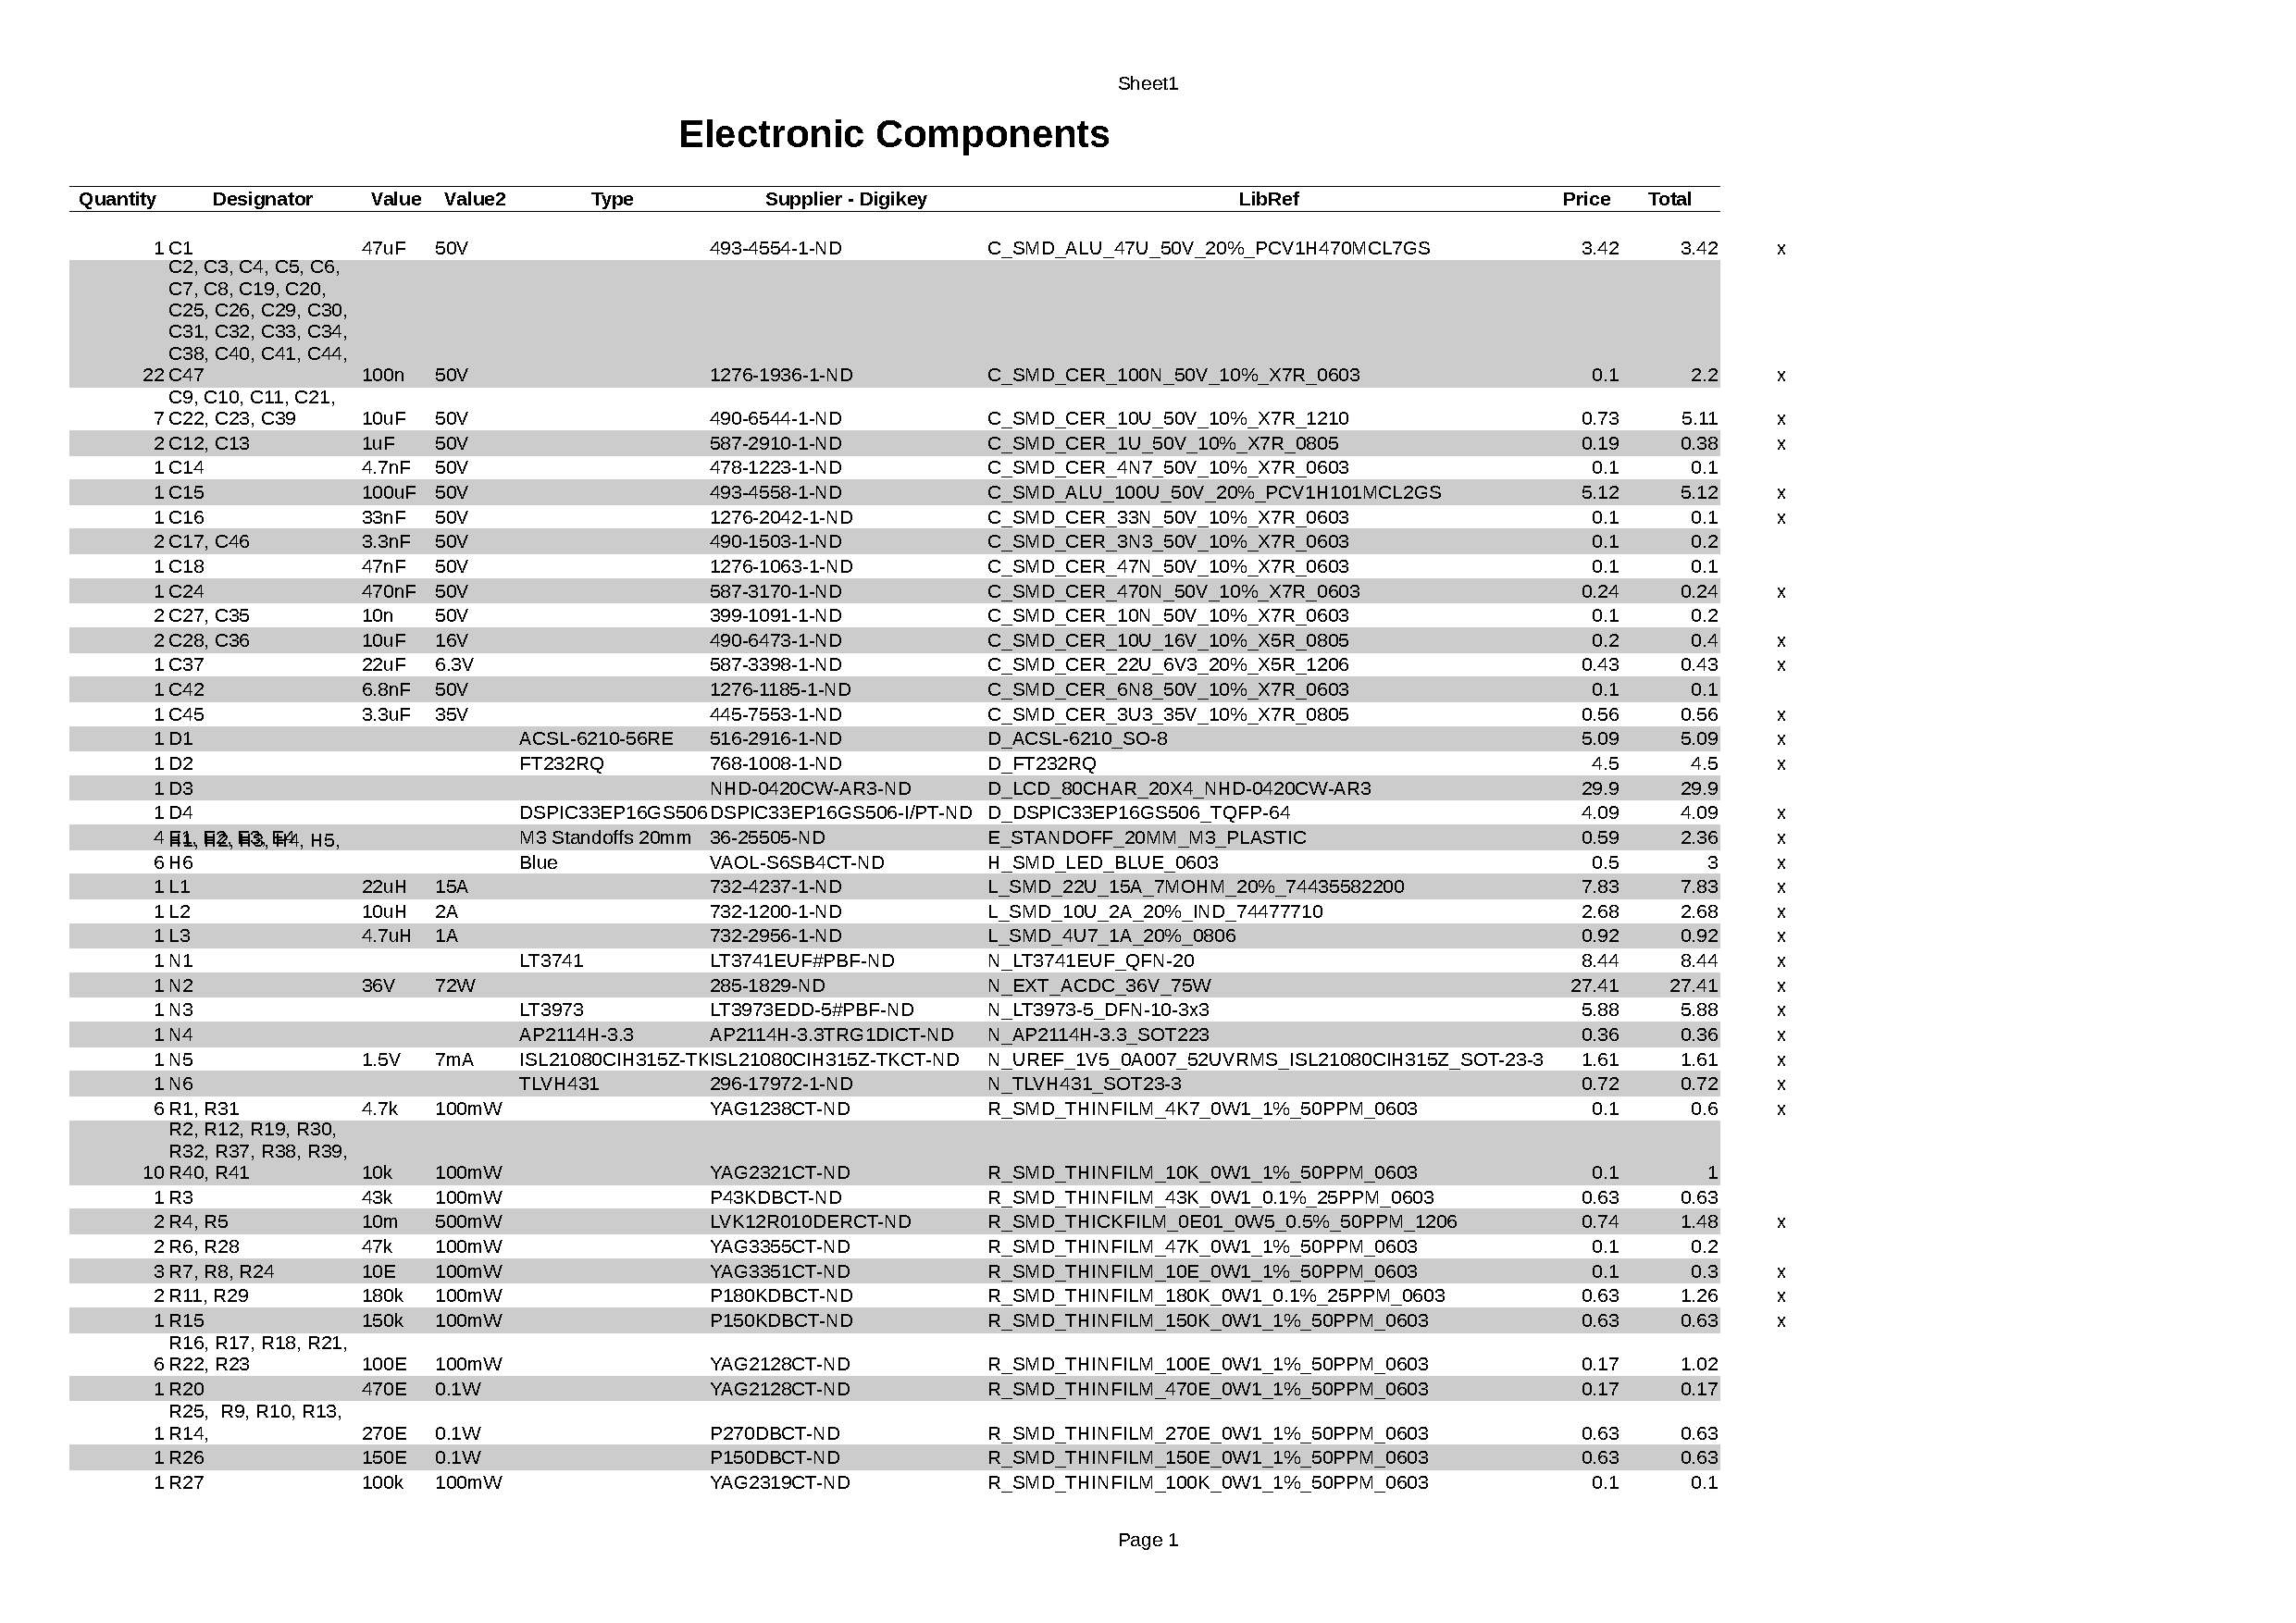
\includepdf[pages=-,scale=1]{images/bom.pdf}


    % **************************************************************************** %
    \section{Circuit Schematics}
    \label{appendix:schematics}
    % **************************************************************************** %
    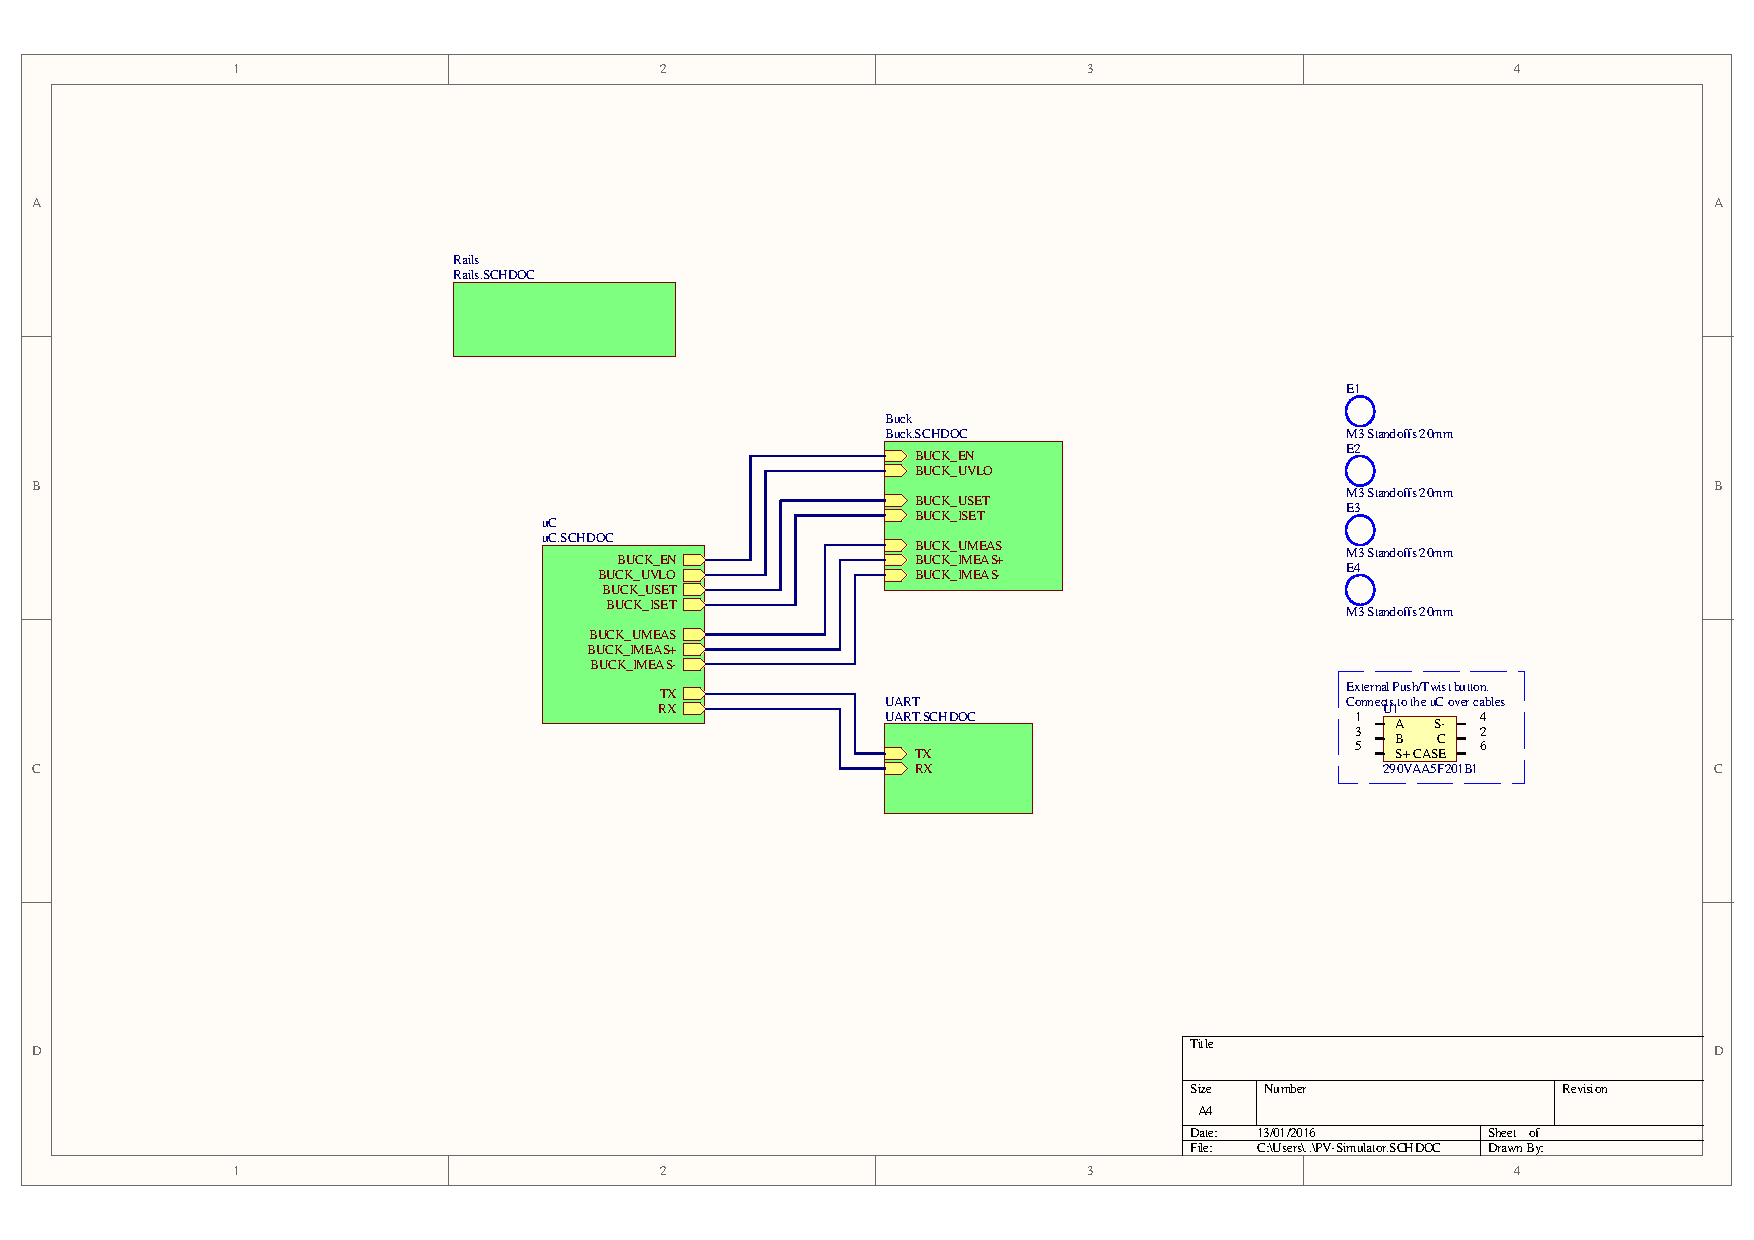
\includepdf[pages=-,scale=1]{images/schematic.pdf}

\setlength\paperheight{210mm}
\setlength\paperwidth{297mm}
\setlength\pdfpageheight{\paperheight}
\setlength\pdfpagewidth{\paperwidth}




% **************************************************************************** %
\clearpage
\section{Inductors}
\label{appendix:inductors}
% **************************************************************************** %

Filtering available  inductors according to  the criteria outlined  in section
\ref{subsubsec:lt3741:inductors} on  page \pageref{subsubsec:lt3741:inductors}
left us  with the models listed  in Table \ref{tab:circuit:buck:inductor}. The
model highlighted  in grey  was selected  due to it  having the  lowest direct
current resistance (DCR).

\begin{table}[th!]
    \begin{center}
        \caption{List of inductors matching our requirements}
        \label{tab:circuit:buck:inductor}
        \begin{tabular}{lcccc}
            \toprule
            Digikey         & Price (CHF) & Inductance (\SI{}{\micro\henry}) & DCR (\SI{}{\ohm}) & Ohmic Loss (\SI{}{\watt}) \\
            \midrule
            \rowcolor{lightgray}
            732-4237-1-ND   & 8.03        & 22                               & 0.007             & 0.175  \\
            732-2179-1-ND   & 6.4         & 47                               & 0.0335            & 0.8375 \\
            732-2177-1-ND   & 6.4         & 22                               & 0.0146            & 0.365  \\
            \bottomrule
        \end{tabular}
    \end{center}
\end{table}


% **************************************************************************** %
\section{MOSFETs}
\label{appendix:mosfets}
% **************************************************************************** %

Table     \ref{tab:circuit:buck:mosfet}     lists    MOSFETs     that     meet
the    constraints     outlined    in     \ref{subsubsec:lt3741:mosfets}    on
\pageref{subsubsec:lt3741:mosfets}.  For each one  the power losses $P_{LOSS}$
and $P_{LOSS\_LDO}$ were calculated.

\begin{table}[th!]
    \begin{center}
        \caption{Possible choices for MOSFETs}
        \label{tab:circuit:buck:mosfet}
        \begin{tabular}{cccccccccc}
            \toprule
            $R_{DS_{(on)}}$ & $Q_{GD}$ & $Q_{GS}$ & $R_G$ & $V_{GS_{THR}}$ & Ohmic Loss & Transision Loss & Total Loss & Drive Loss \\
            \midrule
            0.0032          & 4        & 2.5      & 0.4   & 2.5            & 0.104      & 1.0296          & 1.1336     & 0.806 \\
            0.0039          & 7        & 9        & 2.4   & 3.3            & 0.12675    & 4.8384          & 4.96515    & 1.984 \\
            0.0042          & 7        & 9        & 2.4   & 3.3            & 0.1365     & 4.8384          & 4.9749     & 1.984 \\
            0.008           & 2        & 4.5      & 3     & 2              & 0.26       & 2.2464          & 2.5064     & 0.558 \\
            0.0067          & 5.3      & 3.9      & 1.5   & 1              & 0.21775    & 2.18592         & 2.40367    & 0.7998 \\
            \rowcolor{lightgray}
            0.0093          & 2        & 4.9      & 1     & 2              & 0.30225    & 1.39104         & 1.69329    & 1.488 \\
            0.019           & 8        & 4        & 1.3   & 2              & 0.6175     & 2.6784          & 3.2959     & 1.798 \\
            0.0095          & 7.5      & 6        & 1     & 3              & 0.30875    & 2.7216          & 3.03035    & 1.736 \\
            \bottomrule
        \end{tabular}
    \end{center}
\end{table}


The MOSFET highlighted in grey was selected.  Though it is not the best model,
it is a lot  cheaper than the best fit and  has better documentation. The same
MOSFET is used for both the low-side and the high-side switch.

